\documentclass{article}
\usepackage{polski}
\usepackage[utf8]{inputenc}
\usepackage{listings}
\usepackage{graphicx}
\usepackage{amsmath}  % dla matematycznych symboli

\title{AiSD Lista 2}
\author{Dominik Kowalczyk}

\begin{document}
	\maketitle

\section{Algorytm sortowania QUICKSORT (sortowanie szybkie)}

\large{Do prawidłowej implementacji algorytmu QUICKSORT potrzebna jest funkcja pomocnicza PARTITION, oraz funkcja główna QUICKSORT. W podstawowej wersji kod wygląda następująco:}
\\

\begin{lstlisting}[language=C++, caption={Kod funkcji sortowania szybkiego}, numbers=left, frame=single, xleftmargin=20pt]
int PARTITION(float A[], int p, int r) {
	float x = A[r];
	int i = p - 1;
	
	for (int j = p; j <= r - 1; j++) {
		if (A[j] <= x) {
			i = i + 1;
			float temp = A[i];
			A[i] = A[j];
			A[j] = temp;
		}
	}
	float temp = A[i + 1];
	A[i + 1] = A[r];
	A[r] = temp;
	return i + 1;
}
\end{lstlisting}

\large{W funkcji Partition jako argumenty przyjmujemy tablicę liczb zmiennoprzecinkowych oraz indeksy początku p oraz końca r. Używamy pivota, którym jest nasz \(x\) któremu przypisujemy wartość ostatnią z tablicy (\(A[r]\)). Ustawiamy również indeks i, który będzie rozdzielał części posortowane od nieposortowanej. Następnie przechodzimy do pętli:}

\begin{itemize}
\item \texttt{for (int j = p; j <= r - 1; j++)} \\
Inicjuje pętlę, która iteruje od pierwszego elementu do $r -1$ tablicy $A[1]$. \\


\item \texttt{if (A[j] <= x)} \\
Sprawdzamy, czy nasz pivot jest większy od aktualnie sprawdzanej wartości. Jeśli jest to przesuwamy indeks naszej granicy o jeden w prawo  $i=i+1$ oraz zamieniamy naszą badany element z następnym w kolejności (w kodzie używamy zmiennej tymczasowej, aby nie utracić naszego elementu).
\end{itemize}

\large{Gdy, pętla przestanie działać, czyli pozostałem elementy są większe od naszego aktualnego pivota, otrzymujemy podział na dwie podtablice a nasz pivot zamieniamy z elementem o indeksie za naszą granicą.}
\\

\begin{lstlisting}[language=C++, caption={Kod funkcji sortowania szybkiego}, numbers=left, frame=single, xleftmargin=20pt]
void QUICK_SORT(float A[], int p, int r) {
	if (p < r) {
		int s = PARTITION(A, p, r);
		QUICK_SORT(A, p, s - 1);
		QUICK_SORT(A, s + 1, r);
	}
}
\end{lstlisting}

\large{We właściwej funkcji QUICKSORTA mamy pętle if, w której z naszego podział tablicy z funkcji pomocniczej PARTITION bierzemy i przypisujemy indeks $s$ i dzielimy na jego podstawie na dwie podtablice, które sortujemy rekurencyjnie.}

\newpage

\large{Modyfikacja do algorytmu QUICKSORT (sortowania szybkiego) polega na dzieleniu tablicy na przy pomocy dwóch elementów (na 3 części).}

\begin{lstlisting}[language=C++, caption={Kod funkcji sortowania szybkiego z modyfikacją}, numbers=left, frame=single, xleftmargin=20pt]
float p1 = A[lewy];
float p2 = A[prawy];

if (p1 > p2) {
	swap(A[lewy], A[prawy]);
	p1 = A[lewy];
	p2 = A[prawy];
}

int L = lewy + 1;
int S = lewy + 1;
int P = prawy - 1;
\end{lstlisting}

\large{W przypadku modyfikacji mamy dwa pivoty $p1$ oraz $p2$ gdzie $lewy$ oznacza pierwszy element tablicy (z lewej strony) a $prawy$ ostatni. Następnie mamy pętle porównującą wartości pivotów i jeśli jest taka potrzeba zamienia je miejscami (większy z nic - na końcu tablicy, mniejszy na początku.}
\\

\large{Mamy również trzy nowe zmienne $L$ (element drugi (pierwszy rozpatrywany po pominięciu pivota)), $S$ (aktualnie rozpatrywany element) oraz $P$ (element przedostatni (ostatni przy pominięciu pivota)).}

\begin{lstlisting}[language=C++, caption={Kod funkcji sortowania szybkiego z modyfikacją}, numbers=left, frame=single, xleftmargin=20pt]
while (S <= P) {
	if (A[S] < p1) {
		swap(A[S], A[L]);
		L++;
	} else if (A[S] >= p1 && A[S] <= p2) {
	} else	{
		while (A[P] > p2 && S < P) 
		P--;
		swap(A[S], A[P]);
		P--;
		if (A[S] < p1) {
			swap(A[S], A[L]);
			L++;
		}
	}
	S++;
}
\end{lstlisting}

\large{W powyższym kodzie mamy parę kluczowych pętli:}

\begin{itemize}
\item \texttt{if (A[S] < p1)} \\
Jeśli nasz obecnie sprawdzany element jest mniejszy od naszego pierwszego pivota to $swap(A[S], A[L]);$ - zamienimy miejscami nasz aktualny element z pierwszym elementem w tablicy i przesuwamy naszą granicę w prawo ($L++$).

\item \texttt{else if (A[S] >= p1 "and" A[S] <= p2)} \\
Wartość naszego sprawdzanego elementu jest pomiędzy wartością $p1$ a $p2$, zatem jest we właściwym miejscu - nic nie robimy. (linijka zawarta w kodzie głównie, aby zliczać porównanie).

\item \texttt{while (A[P] > p2 "and" S < P)} \\
Tutaj rozpatrujemy przypadek, w którym nasz badany element jest większy od drugiego pivota. Wtedy (za sprawą pętli while) szukamy elementu, który jest mniejszy od większego z pivotów i przesuwamy go do środkowej części, zmniejszając prawą granicę w lewo. Zamieniamy rozpatrywany element z tym znalezionym z poprzedniej pętli i znowu idziemy z prawą granicą w lewo. Jeśli nasz nowy rozpatrywany element jest mniejszy od naszego mniejszego z pivotów to przenosimy go do części dla elementów mniejszych od $p1$ i idziemy z granicą lewą granicą w prawo. 
\end{itemize} 

\large{Funkcja główna jest już mało ciekawa, gdyż różnic się od wersji bez modyfikacji tylko tym, że mamy jeden dodatkowy obszar do rozważenia przy sortowaniu rekurencyjnym. }

\newpage

\section{Algorytm sortowania RADIXSORT (z użyciem COUNTINGSORT)}

\large{Sortowanie pozycyjne jesteśmy w stanie zaimplementować w oparciu o, między innymi sortowanie przez zliczanie. Zacznijmy od przeanalizowania właśnie jego.}

\begin{lstlisting}[language=C++, caption={Kod funkcji sortowania pozycyjnego}, numbers=left, frame=single, xleftmargin=20pt]
void COUNTINGST(int A[],int n,int exp,int d){
	int* B = new int[n];
	int* C = new int[d]();
	
	for (int i = 0; i < n; i++) {
		int j = (A[i] / exp) % d;
		C[j]++;
	}
	
	for (int i = 1; i < d; i++) {
		C[i] += C[i - 1];
	}
	
	for (int i = n - 1; i >= 0; i--) {
		int j = (A[i] / exp) % d;
		B[C[j] - 1] = A[i];
		C[j]--;
	}
	
	for (int i = 0; i < n; i++) {
		A[i] = B[i];
	}
	
	delete[] B;
	delete[] C;
}

\end{lstlisting}

\large{W tym przypadku, jako kod analizę należałoby zaczniemy od wyjaśnienia czym jest exp (wykladnik) i d (podstawa systemu liczbowego). Tworzymy dwie tablica, jedna do przechowywania ilości zliczeń (w naszym wypadku to $C[]$) oraz wynikowa, czyli $B[]$. W pierwszej pętli $for$ wyznaczamy cyfry setek, dziesiątek, jedności, itd. i zapisujemy w tablicy zliczeń. W następnej funkcji sumujemy poprzednie wartości zliczeń, aby prawidłowo wyznaczyć miejsce przypisania do tablicy wynikowej. Umieszczamy wyniki z tablicy C do B (cofając indeks o jeden abyśmy zaczynali od początku B). Na sam koniec przypisujemy wypełnioną tablicę wynikową do tablicy właściwej $A[]$.}

\begin{lstlisting}[language=C++, caption={Kod funkcji sortowania pozycyjnego}, numbers=left, frame=single, xleftmargin=20pt]
void RADIX_SORT(int A[], int n, int d) {
	int maks_war = A[0];
	for (int i = 1; i < n; i++) {
		if (A[i] > maks_war) {
			maks_war = A[i];
		}
	}
	int k = 0;
	while (maks_war > 0) {
		maks_war /= d;
		k++;
	}
	for (int exp = 1, iter = 0; iter < k;
	 exp *= d, iter++) {
		COUNTING_SORT(A, n, exp, d);
	}
}
\end{lstlisting}

\large{W funkcji RADIXSORT na dobrą sprawę niewiele się dzieje. Właściwe to większość funkcji jest wyznaczenie wartości $k$, która reprezentuje maksymalną liczbę cyfr w największej liczbie. Kod jednakowoż to nic innego jak znajdowanie największej liczby w tablicy i zliczenie jej ilości cyfr. Oczywiście w funkcji występuje również wywołanie sortowania przez zliczanie, które przy posiadaniu zmiennej, mamy granicę mówiącą jak długo mamy iterować po zmiennych.}\\

\large{Modyfikacja do RADIXSORTA polega na tym, aby funkcja sortowała liczby całkowite (czyli dodatnie i ujemne) a nie same dodatnie, tak jak mamy w przypadku klasycznego algorytmu.}\\

\large{Mój pomysł na implementację tej modyfikacji jest podzielenie na dwie tablice (oddzielne) liczb ujemnych i dodatnich, po czym dodatnie posortować w taki sam sposób jak w klasycznej wersji algorytmu, a dla ujemnych zmienić znak i również zastosować sprawdzony już kod, posortować odwrócić, przywrócić znak i złączyć obie podtablice.Ze względu na to, że kod jest długi i w większości analogiczny to przedstawię sposób uporządkowania liczb ujemnych.}

\begin{lstlisting}[language=C++, caption={Kod funkcji sortowania pozycyjnego z modyfikacją}, numbers=left, frame=single, xleftmargin=20pt]
void RADIX_SORT_MOD(int A[], int n, int d) {
	int licz_dodatnich = 0;
	int licz_ujemnych = 0;
	
	for (int i = 0; i < n; i++) {
		if (A[i] >= 0) {
			licz_dodatnich++;
		} else {
			licz_ujemnych++;
		}
	}
	int*dodatnie = new int[licz_dodatnich];
	int*ujemne = new int[licz_ujemnych];
	
	int plus = 0;
	int minus = 0;
	
	for (int i = 0; i < n; i++) {
		if (A[i] >= 0) {
			dodatnie[plus++]=A[i];
		} else {
			ujemne[minus++]=-A[i];
		}
	}
}
\end{lstlisting}

\large{W powyższym kodzie, tak jak ostatnio nie mamy nic spektakularnego rozdzielamy na liczby dodatnie i ujemne, tworzymy dla nich dwie osobne tablice i przypisujemy odpowiednie elementy z uwagą, że przy przypisywaniu liczb ujemnych do tablicy zmieniamy ich znak na dodatni.} \\

\begin{lstlisting}[language=C++, caption={Kod funkcji sortowania pozycyjnego z modyfikacją}, numbers=left, frame=single, xleftmargin=20pt]
int max_ujemne = 0;
if (liczba_ujemnych > 0) {
	max_ujemne = ujemne[0];
}
for (int i = 1; i < liczba_ujemnych; i++) {
	if (ujemne[i] > max_ujemne) {
		max_ujemne = ujemne[i];
	}
}

int k_ujemne = 0;
while (max_ujemne > 0) {
	max_ujemne /= d;
	k_ujemne++;
}
\end{lstlisting}

\large{W tym przypadku dostajemy bardzo analogiczny przypadek co w klasycznym RADIXSORCIE. Potrzebujemy określić ilość cyfr w największej i najmniejszej liczbie (bo 500 i -500 może się wydarzyć). Ponownie otrzymujemy wielokrotnie wałkowany w tym sprawozdaniu moment szukania wartości największej i jak wcześniej zliczania cyfr. Następnie sortujemy oddzielnie tablice dodatnie oraz ujemne, łączymy je (z zastrzeżeniem, że najpierw wpisujemy do tablicy właściwej cyfry z podtablicy dla liczb ujemnych ze zmianą znaku, a następnie dodatnie.).}\\


\section{Algorytm sortowanie kubełkowego BUCKETSORT (z użyciem INSERTION SORT)}

\large{Algorytm BUCKET SORT bazuje swoje sortowanie na sortowaniu przez wstawianie zaimplementowane na listach. Przejdźmy najpierw może przez kod INSERTIONSORTA na listach.}
\newpage
\subsection{INSERTIONSORT na listach}

\begin{lstlisting}[language=C++, caption={Kod funkcji sortowania przez wstawianie na listach}, numbers=left, frame=single, xleftmargin=20pt]
struct WEZEL {
	float wartosc;
	WEZEL* prev;
	WEZEL* next;
\end{lstlisting}

\large{Zaczynamy od zainicjowania elementu listy - $WEZEL$, gdzie $wartosc$ przechowuje wartość węzła (liczbę zmiennoprzecinkową). Wyróżniamy również $prev$, który wskazuje na węzeł poprzedni oraz $next$ wskazujący na element następny.}

\begin{lstlisting}[language=C++, caption={Kod funkcji sortowania przez wstawianie na listach}, numbers=left, frame=single, xleftmargin=20pt]
struct LISTA {
	WEZEL* head;
	LISTA() : head(nullptr) {}
\end{lstlisting}

\large{Definiujemy listę jako strukturę danych, do której inicjalizacji używamy "głowy" ($head$), która na początku przechowuje pierwszy element listy. Tworzymy pustą listę.}
\\

\large{Następnie do struktury danych listy dodajemy funkcje określające jej działanie. W skład ich wchodzi funkcja usuwająca element, drukująca listę, czy szukająca elementu, jednak najciekawsza z nich jest funkcja dodająca element do listy.}

\begin{lstlisting}[language=C++, caption={Kod funkcji sortowania przez wstawianie na listach}, numbers=left, frame=single, xleftmargin=20pt]

void LIST_INSERT(LISTA& lista, WEZEL* x) {
	x->next = lista.head;
	x->prev = nullptr;
	if (lista.head == nullptr) {
		lista.head = x;
	} else {
		lista.head->prev = x;
		lista.head = x;
	}
}
\end{lstlisting}

\large{Ustawiamy nowy element listy na po nim następujący ($next$), gdyż świeżo dodany element będzie na pierwszym miejscu. Nowy węzeł oczywiście nie ma poprzednika, stąd $x->prev = nullptr$. Jeśli lista jest pusta ustawiamy "głowę" na $x$ bo jest to nasz jedyny element. W przeciwnym wypadku ustawiamy poprzednik listy na nasz $x$ w celu połączenia nowego węzła z listą i przestawiamy na niego "głowę" bo to naturalnie pierwszy element listy.
	
\begin{lstlisting}[language=C++, caption={Kod funkcji sortowania przez wstawianie na listach}, numbers=left, frame=single, xleftmargin=20pt]
void LIST_INSERTION_SORT(LISTA& l) {
	WEZEL* element = l.head->next;
	while (element != nullptr) {
		float key = element->wartosc;
		WEZEL* prev = element->prev;
		while (prev != nullptr &&
			prev->wartosc > key) {
			
			prev->next->wartosc =
			prev->wartosc;
			
			prev = prev->prev;
		}
		
		if (prev == nullptr) {
			l.head->wartosc = key;
		} else {
			prev->next->
			wartosc=key;
		}
		
		element = element->next;
	}
}
\end{lstlisting}

\large{Wiedząc, że lista nie jest pusta, możemy posortować ją przy pomocy powyżeszego sortowania przez wstawianie, które działa ideowo tak samo jak ten na tablicach, przy czym tam przesuwaliśmy indeksy, to przesuwamy o węzły. Podobnie mamy klucz : $key$, która przechowuje aktualna wartosc naszego elementu. Rozpoczynamy od drugiego elementu i kierujemy się w lewo listy. Pętla while ma za zadanie umiejscowienie na odpowiednie miejsce naszego klucza przesuwając węzły. Schemat działania pod tym względem identyczny, doskonale znany.}

\subsection{BUCKET SORT}

\large{Mając napisany INSERTION SORT na listach możemy bez problemowo przejść do implementacji sortowania kubełkowego.}

\begin{lstlisting}[language=C++, caption={Kod funkcji sortowania kubełkowego}, numbers=left, frame=single, xleftmargin=5pt, xrightmargin=5pt]
void BUCKET_SORT(float* A, int n) {
	LISTA* B = new LISTA[n];
	
	for (int j = 0; j < n; j++) {
		B[j] = LISTA();
	}
	for (int i = 0; i < n; i++) {
		int in=static_cast<int>(n*A[i]);
		WEZEL*nwezel = new WEZEL(A[i]);
		B[in].LIST_INSERT(B[in],nwezel);
	}
	for (int j = 0; j < n; j++) {
		B[j].LIST_INSERTION_SORT(B[j]);
	}
	int s = 0;
	for (int j = 0; j < n; j++) {
		WEZEL* elem = B[j].head;
		while (elem != nullptr) {
			A[s++] = elem->wartosc;
			elem = elem->next;
		}
	}
	delete[] B;
}
\end{lstlisting}

\large{Tworzymy tablicę pomocniczą B, która przechowuje początkowo puste listy.}
\begin{itemize}
	\item Operacje w pierwszej pętli for:
	\begin{itemize}
		\item Obliczenie indeksu koszyka: \[ \texttt{int in = static\_cast<int>(n * A[i]);} \]
		\item Utworzenie nowego węzła z wartością: \[ \texttt{WEZEL* nwezel = new WEZEL(A[i]);} \]
		\item Dodanie elementu do odpowiedniego koszyka: \[ \texttt{B[in].LIST\_INSERT(B[in], nwezel);} \]
	\end{itemize}
\end{itemize}

\begin{itemize}
	\item Sortowanie list w każdym koszyku:
	\begin{itemize}
		\item Iteracja po koszykach: \texttt{for (int j = 0; j < n; j++)}
		\item Sortowanie listy w koszyku: \[ \texttt{B[j].LIST\_INSERTION\_SORT(B[j]);} \]
	\end{itemize}
	\item Przenoszenie posortowanych elementów z koszyków do tablicy \texttt{A}:
	\begin{itemize}
		\item Inicjalizacja indeksu: \[ \texttt{int s = 0;} \]
		\item Iteracja po koszykach: \texttt{for (int j = 0; j < n; j++)}
		\item Iteracja po elementach w koszyku:
		\begin{itemize}
			\item Pobranie pierwszego elementu: \[ \texttt{WEZEL* elem = B[j].head;} \]
			\item Przechodzenie przez listę:
			\begin{itemize}
				\item Przypisanie wartości z elementu do \texttt{A}: \[ \texttt{A[s++] = elem->wartosc;} \]
				\item Przejście do następnego elementu: \[ \texttt{elem = elem->next;} \]
			\end{itemize}
		\end{itemize}
	\end{itemize}
\end{itemize}

\newpage

\large{Modyfikacja BUCKETSORT ma polegać na tym, aby algorytm sortował dla dowolnych danych wejściowych.Jednakowoż działa on bardzo w analogiczny sposób gdyż moja implementacja ten modyfikacji polega na zmianie numeracji, normalizacji kubełków.}

\begin{lstlisting}[language=C++, caption={Kod funkcji sortowania kubełkowego z modyfikacją}, numbers=left, frame=single, xleftmargin=5pt, xrightmargin=5pt]
void BUCKET_SORT_MOD(float A[], int n) {
	float min = A[0];
	float max = A[0];
	
	for (int i = 1; i < n; i++) {
		if (A[i] < min) {
			minimum = A[i];
		}
		if (A[i] > max) {
			max = A[i];
		}
	}
	
	if (max == min) {
		for (int i = 0; i < n; i++) {
			A[i] = min;
		}
		return;
	}
}
\end{lstlisting}

\large{Początkowo znajdujemy wartość maksymalną oraz minimalną, aby mieć punkt odniesienia do skalowania wartości kubełków.}

\begin{lstlisting}[language=C++, caption={Kod funkcji sortowania kubełkowego z modyfikacją}, numbers=left, frame=single, xleftmargin=5pt, xrightmargin=5pt]
for (int i = 0; i < n; i++) {
	int index = static_cast<int>
	(n * (A[i] - min) / (max - min));
	
	if (index == n) {
		index = n - 1;
	}
}
\end{lstlisting}

\large{Dzięki odnalezieniu wartości maksymalnej oraz minimalnej jesteśmy w stanie zmodyfikować sprawdzaną wartość na liczbę z przedziału od $0$ do $1$. Pozostała część kodu jest identyczna jak przy normalnym sortowaniu kubełkowym.}

\section{Porównania algorytmów}
\subsection{QUICKSORT VS BUCKETSORT}
	
\begin{figure}[h]
	\centering
	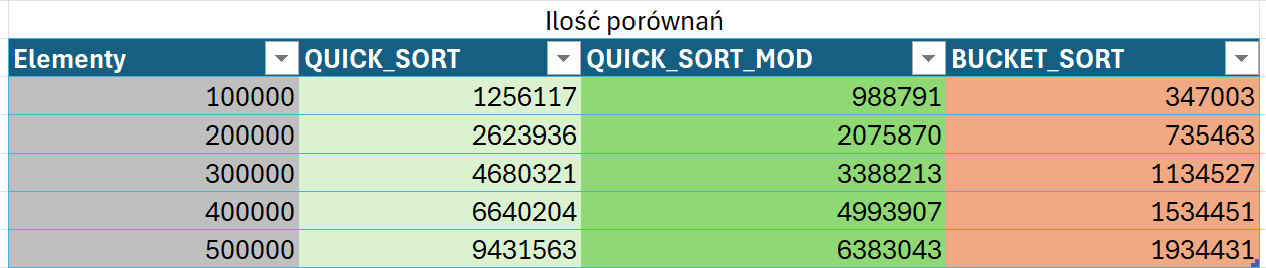
\includegraphics[width=1\textwidth]{porownania.png}
	\caption{Tabela ilości porównań  w QUICKSORT, QUICKSORT MOD i BUCKETSORT.}
	\label{fig:table1}
\end{figure}
	
\begin{figure}[h]
	\centering
	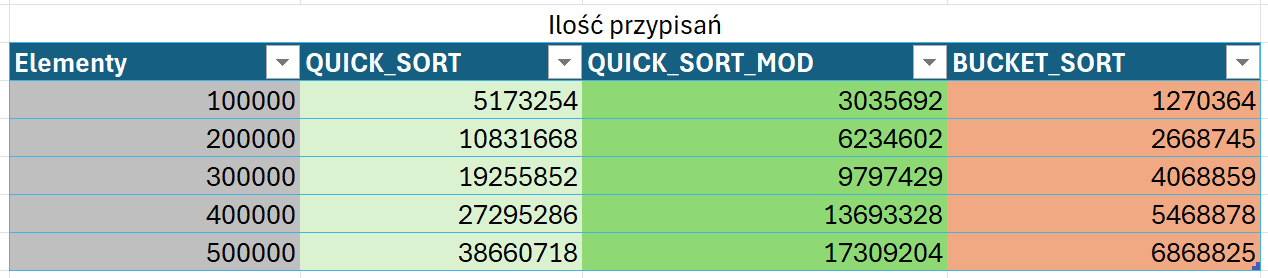
\includegraphics[width=1\textwidth]{przypisania.png}
	\caption{Tabela ilości przypisań  w QUICKSORT, QUICKSORT MOD i BUCKETSORT.}
	\label{fig:table2}
\end{figure}

\begin{figure}[h]
	\centering
	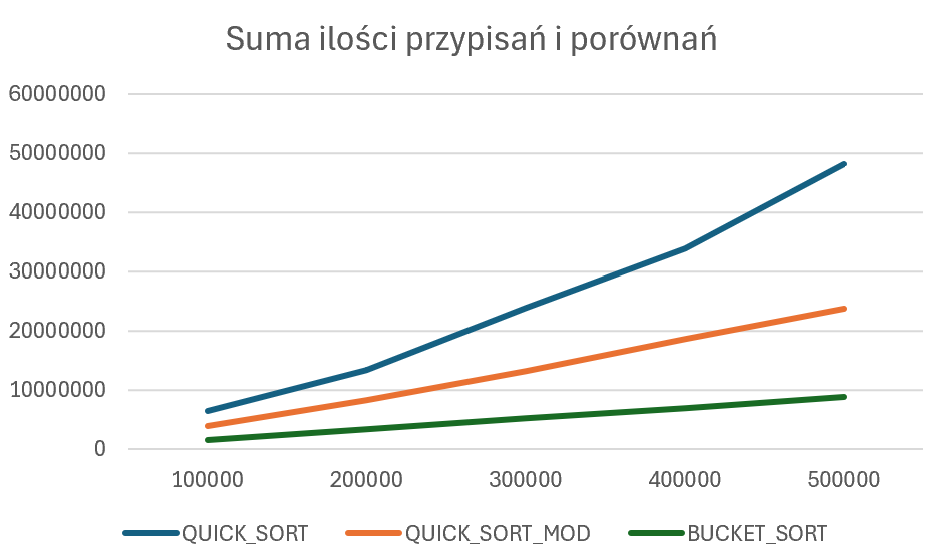
\includegraphics[width=1\textwidth]{wykres.png}
	\caption{Wykres sumy przypisań i porównań  w QUICKSORT, QUICKSORT MOD i BUCKETSORT.}
	\label{fig:wykres2}
\end{figure}

\begin{figure}[h]
	\centering
	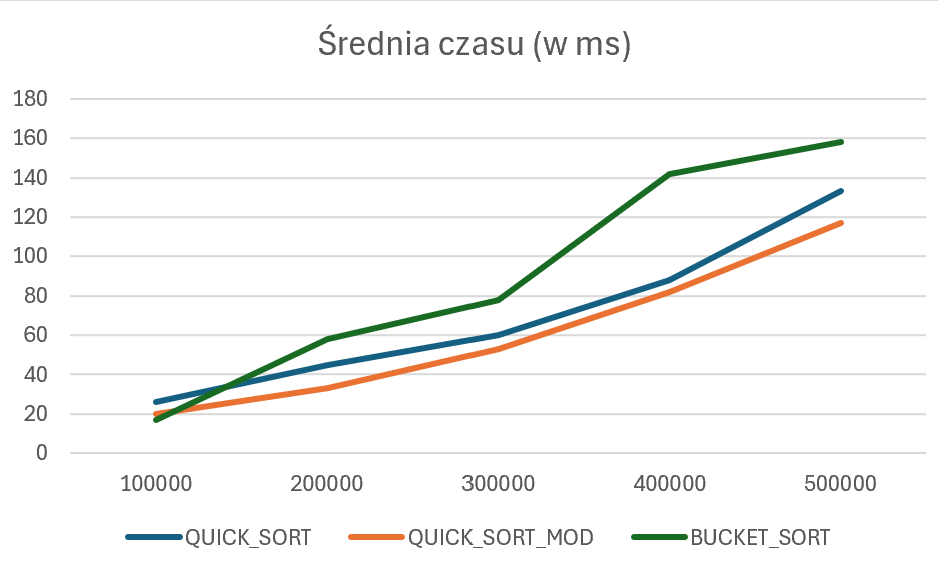
\includegraphics[width=1\textwidth]{czas.png}
	\caption{Wykres czasu działania   QUICKSORT, QUICKSORT MOD i BUCKETSORT.}
	\label{fig:wykres1}
\end{figure}

\large{Pod względem złożoności obliczeniowej, możemy powiedzieć, że najlżejszym algorytmem jest ewidentnie BUCKETSORT. Wykres wygląda jakby był liniowy i zgadza się to z założeniem teoretycznym jako, że ma on złożoność obliczeniową $O(n)$. Drugim poz względem złożoności będzie QUICKSORT MOD, który na w miarę wydłużania się listy, coraz bardziej oddalał się od normalnego QUICKSORTA. W tym przypadku również możemy wywnioskować złożoność, gdyż wykres sugeruje nam, że QUICKSORT będzie $O(n^2)$, a zmodyfikowany $O(n \log n)$, co również pokrywa się ze stroną teoretyczną.}

\large{Jeśli jednak patrzymy na wydajność, złożoność czasową, to najkrócej działającym algoytmem jest zmodyfikowany QUICKSORT, a zdecydowanie najwolniejszym BUCKETSORT.}



\end{document}